\documentclass[12pt]{article}
\usepackage{setspace}
%\doublespacing

\usepackage{threeparttable}  
\usepackage{graphicx}
\usepackage{subcaption}
\usepackage[margin=1in]{geometry}
\usepackage[backend=bibtex,style=authoryear]{biblatex}
\addbibresource{sdsa_brief.bib}
\usepackage[colorlinks=true,
            linkcolor=blue,
            urlcolor=blue,
            citecolor=blue]{hyperref}
\usepackage{tabularx}
\usepackage{array}        
\usepackage{footnote}  
\usepackage{amsmath}
\usepackage{comment}
\usepackage{booktabs}
\usepackage{siunitx}
\usepackage[section]{placeins}
\makeatletter
\AtBeginDocument{%
  \expandafter\renewcommand\expandafter\subsection\expandafter
    {\expandafter\@fb@secFB\subsection}%
}
\makeatother
\sisetup{detect-weight=true,detect-family=true}

\makesavenoteenv{tabularx}  

\graphicspath{{output/figures/}}

\title{A Stochastic Framework for U.S. Debt Sustainability}
\author{Jared Bernstein, Daniel Posthumus, Adam Shaw}

\begin{document}

\maketitle

\section{Introduction}

In our \href{https://siepr.stanford.edu/publications/policy-brief/us-budget-math-looking-dangerous}{previous paper} on the U.S. fiscal outlook, we warned that the ``math is looking dangerous.'' We showed that conditions formerly favorable to debt sustainability, most notably $r < g$ (the debt's interest rate being lower than the economy's growth rate), have deteriorated in recent years as rates rose and growth slowed. We also argued that debt sustainability and the trajectory of the debt had been worsened by Congressional actions that financed historically large tax cuts and spending through deficits. For example, the recently-passed One Big Beautiful Bill Act (OBBBA), according to the \href{https://budgetlab.yale.edu/research/long-term-impacts-one-big-beautiful-bill-act-enacted-july-4-2025}{Yale Budget Lab}, will raise the debt-to-GDP ratio by 52 percentage points from its baseline in 30 years.

One challenge in the debt sustainability literature is that there is no single, widely-accepted metric (by academics and policymakers alike) to distinguish the sustainability of one budget path relative to another. Historically large increases in debt-to-GDP ratios are certainly a signal of rising fiscal vulnerability; however, numerous countries --- Japan is an oft-cited example --- have experienced such increases in their debt-to-GDP ratio without the kind of acute market stress about which ``budget hawks'' typically warn. 

We therefore introduced a new warning criterion for unsustainability: ``ahistorical adjustments'' (AA), meaning a situation where external factors --- such as a sharp rise in term premia on government debt --- necessitate a drastic, sudden adjustment to discretionary fiscal policy, i.e., primary deficit reductions. When that adjustment is ``large'' in historical terms we argued that the path is potentially unsustainable. Here, we take a step towards formalizing and quantifying this definition.

In this paper, we build a stylized stochastic model to more rigorously identify the factors that determine debt sustainability and what constitutes an AA. This model takes external projections of the basic determinants of debt and, through stochastic laws of motion, produces a distribution of fiscal outcomes. The model is deliberately non-structural; assumptions are both transparent and adjustable to policymakers. Within this model, we are able to simulate and transparently alter assumptions around (1) Congress's policy responsiveness to the fiscal outlook; (2) the persistence over time and projected path of interest rates; and --- most importantly --- (3) alternative assumptions about the mean future path of growth, interest rates, and the primary deficit. In this paper, we present one such example of using the model to evaluate alternative futures, focusing on AI-driven productivity growth counterfactuals. In an accompanying policy memo, we present a streamlined presentation of these findings --- illustrating our model's tractability and capacity to contribute to policy discussions.

\section{Developing a Model of Debt}

To formalize and quantify ahistorical adjustments (AA), we construct a model. The model we build is a variation of a class of probabilistic models known as Stochastic Debt Sustainability Analysis (SDSA), as in \href{https://direct.mit.edu/books/oa-monograph/5522/Fiscal-Policy-under-Low-Interest-Rates}{Blanchard} (2024) and \href{https://didattica.unibocconi.it/mypage/dwload.php?nomefile=Fiscal_Macro_2025_(3)20250403120402.pdf}{Favero} (2025). We use a set of stochastic laws of motion to simulate paths for the relevant determinants of $b$, the ratio of debt held by the public to GDP: primarily $r$, $g$, and $s$ (the real interest rate, real growth rate, and primary balance, respectively).\footnote{See \textcite{celasun_2006}; \textcite{cottarelli_2011}; \textcite{berti_2013}; \textcite{demirel_2022}; and \textcite{auerbach2025robust}. Celasun and Ostry (2006), employing a ``fan chart'' approach, were particularly pioneering for introducing a probabilistic approach to the then-standard debt sustainability framework of ``deterministic bound-testing''. The primary motivation for opting for a probabilistic approach is that we don't rely on a few stylized exogenous shocks to generate a range of outcomes, allowing for greater flexibility and higher fidelity.}  With this framework, we want to build a model that can be useful to policymakers considering measures that would change the fiscal path. Accordingly, we focus on tractability and transparency. Ours is a similar approach to the IMF's \href{https://www.imf.org/en/Publications/DSA/sovereign-risk-and-debt-sustainability-analysis-for-market-access-countries}{Sovereign Risk and Debt Sustainability Analysis for Market Access Countries} and the European Commission's \href{https://economy-finance.ec.europa.eu/publications/debt-sustainability-monitor-2024_en}{Debt Sustainability Monitor}.

We develop the system of equations \ref{eq:sdsa_debt}-\ref{eq:sdsa_average_interest}. Together, they generate a distribution of future debt paths via Monte Carlo simulations. The remainder of this section explains these equations and their logic.
\begin{gather}
	    b_t = b_{t-1} + \frac{r_t^{av} - g_t}{1 + g_t} b_{t-1} - s_t
        \label{eq:sdsa_debt} \\
        s_t = (1 - c)a_{st} + c\left(\frac{r_t^{av} - g_t}{1 + g_t}\right) b_{t-1} + e_t^s,\quad e_t^s \sim \mathcal{N}(0, \sigma^2_s)
        \label{eq:sdsa_deficit} \\
        g_t = a_{gt} + x_{gt} + e^g_t,\quad e^g_t \sim \mathcal{N}(0, \sigma^2_g)
        \label{eq:sdsa_growth} \\
        x_{gt} = x_{g,t-1} + e^x_t,\quad e^x_t \sim \mathcal{N}(0, \sigma^2_x)
        \label{eq:sdsa_growth_persistent} \\
        r_t = a_{rt} + z_t
        \label{eq:sdsa_interest} \\
        \Delta z_t = \beta_r (\Delta b^s_{t-1} - \rho \Delta b^s_{t-2}) + \rho \Delta z_{t-1} + (e^r_t - e^r_{t-1}),\quad e^r_t \sim \mathcal{N}(0, \sigma^2_r)
        \label{eq:sdsa_interest_deviations} \\
        r_t^{av} = \sigma \cdot r^{av}_{t-1} + (1 - \sigma) \cdot r_t
        \label{eq:sdsa_average_interest} 
\end{gather}
where $b_t$ is the debt-to-GDP (ratio), $g_t$ is the real GDP growth rate, $s_t$ is the primary balance (surpluses appearing as positive), $r_t$ is the long-term real rate (effectively the real 10-year interest rate), and $r^{av}_t$ is the average effective real rate on outstanding debt --- all indexed by year $t$. Unless otherwise noted, all interest and growth rates in this paper are real (inflation-adjusted) annual rates.

Within this framework, we add two concepts. Here we define a debt-stabilizing primary balance, $s^{\text{stab}}_t$ and the stabilizing adjustment, $AA_t$:
\begin{gather}
    s^{\text{stab}}_t = \frac{r_t^{av} - g_t}{1 + g_t} b_{t-1} 
    \label{eq:stab_balance} \\
    AA_t = s^{\text{stab}}_t - s_t
    \label{eq:adjustment}
\end{gather} 
Note that, absent fiscal shocks ($e_t^s = 0$), the stabilizing primary balance equals the primary balance in year $t$ if Congress became 100\% responsive (i.e., $c=1$). We interpret $AA_t$ as the one-period primary-balance tightening (in percent of GDP) that would be required in year $t$ to stabilize the debt ratio given realized interest-growth conditions. With the primary balance defined as positive in surplus, $AA_t>0$ implies a required fiscal tightening, while $AA_t \leq 0$ implies no tightening is required for stabilization in that year.

\subsection{Our Approach to Modeling the Interest Rate $r$}
This subsection provides an overview of how we model $r$; for more details, see Appendix Subsection \ref{sec:detailed_explanation_r}. We model two separate interest rates: the market interest rate, $r_t$, and the average effective rate on outstanding debt, $r^{av}_t$. $r^{av}_t$ directly affects debt accumulation; $r_t$, the contemporaneous rate of newly issued debt, gradually shapes $r^{av}_t$.

We model the market interest rate in two steps. First, we start with CBO's baseline projection for the 10-year real interest rate. Like our modeling methodology of the model's other core inputs, CBO's baseline projection, $a_{rt}$, is the mean interest rate path. Then to this baseline we add a $z_{rt}$, which captures deviation from CBO's baseline due to other shocks in the model feeding into extraneous interest rate changes. We initialize $z_t$ to equal 0 in the first period; starting with the first period, the path of $z_t$ is governed by the law of motion expressed in Equation \ref{eq:sdsa_interest_deviations}. Note that the CBO rate path is roughly consistent, particularly in the long run, with post-GFC estimates of the neutral real rate ($r^* \approx 1\%)$). 

We allow for the market interest rate to deviate from CBO's baseline in two ways. First, we model \textbf{surprise} changes in the debt. These we model as $\Delta b^s_t = \Delta b_t - \Delta b^{CBO}_t$; by differencing out the CBO-implied changes in the debt, we avoid double-counting the feedback effects already baked into CBO baseline projections for the interest rate.\footnote{$\Delta b^{CBO}_t$ is estimated from a deterministic (i.e., no shocks) run of the model using CBO's baseline projections for growth, interest rates, and primary balance and $c = 0$ (i.e., no fiscal policymaking response to debt accumulation). \\ The application of $\beta_r$ here assumes that the marginal feedback effect on the term premium is the same for expected and surprise increases in debt. We view this is a conservative assumption.} Second, we adopt a stochastic innovation term, $(e^r_t - e^r_{t-1})$. This yields the following law of motion for modeling the surprise changes in debt:
\begin{gather}
        \Delta z_t = \beta_r (\Delta b^s_{t-1} - \rho \Delta b^s_{t-2}) + \rho \Delta z_{t-1} + (e^r_t - e^r_{t-1}),\quad e^r_t \sim \mathcal{N}(0, \sigma^2_r)
\end{gather}

This setup requires the estimation of $\beta_r$ and $\rho$. $\beta_r$ governs the magnitude of the pass-through effect of changes in debt on changes in the interest rate while $\rho$ governs the persistence of interest rate deviations from the baseline. Our estimation strategy for these parameters, relying on first-differencing to avoid our model being overcome by the secular downward trend in the term premium and upwards trend in the debt level, mirrors that of \textcite{gust2024government}. We estimate the following equation:
\begin{gather}
    \Delta y_t = \beta_r \Delta b_{t-1} - \beta_r \rho \Delta b_{t-2} + \rho \Delta y_{t-1} + \gamma ' \Delta \mathbf{X_t} + \epsilon_t,
    \label{eq:r_estimation}
\end{gather}
where $y_t$ is the 10-year ACM term premium \parencite{adrian_2012} --- which we use as a proxy for the component of long-term interest rates plausibly affected by debt supply, $b_t$ is the ratio of publicly-held debt to GDP, and $\mathbf{X_t}$ a vector of controls (we keep this lean to avoid overfitting in our model, so that only output gap and the ratio of the primary balance to GDP, $s_t$, are included).\footnote{The term premium is in percentage points, debt is expressed as a percent of GDP, and all $\Delta$ values are quarter-to-quarter changes in percentage points. Thus $\beta_r$ should be interpreted as the effect of a one percentage point quarterly change in the debt as a percentage of GDP on the term premium.} Then, we set $\rho$ to be equal to the coefficient on $\Delta y_{t-1}$.\footnote{Specifically, we estimate Equation \ref{eq:r_estimation} via Ordinary-Least-Squares (OLS) with Newey-West HAC standard errors.} The full results from estimating Equation \ref{eq:r_estimation} can be found in Table \ref{tab:r_estimation_results}. 

The results, which are robust to splitting the sample around the GFC, show that $\hat{\beta_r} = 0.017$ --- meaning a one percentage point quarterly increase in the debt as a percentage of GDP will translate to a 1.7 basis point increase in the term premium --- and $\hat{\rho} = 0.158$. This estimate of $\hat{\beta_r}$ falls within the historical estimates for the parameter (for a range of previous estimates of $\beta_r$, see Table \ref{tab:debt_gdp_interest_effect} in the Appendix), toward the lower end of the distribution of prior estimates. This suggests that, in effect, our debt projections should be interpreted as lower bounds; a higher value for $\hat{\beta}_r$ would amplify any modeled debt path. We use these values of $\hat{\rho}$ and $\hat{\beta}_r$ when running our SDSA Monte Carlo simulations. While $\hat{\rho}$ and $\hat{\beta}_r$ are estimated at the quarterly frequency, to be clear, as a calibration, we are applying them to annualized dynamics in simulations.\footnote{This is valid for $\beta_r$ because feedback effects between quarterly changes in debt and quarterly changes in term premiums should not significantly diverge with the feedback effects between annual changes in debt and annual changes in term premiums. For $\rho$, the application of our quarterly estimate to the annual frequency very likely overstates persistence, making our projections conservative.}

Lastly, we need to model the market rate's feeding into the average effective rate on outstanding debt, $r^{av}_t$. This requires us to fix $\sigma$; here we use $\sigma = 0.8$, which suggests that in each period 20\% of the debt is subject to fluctuations in the market real interest rate.\footnote{In practice, $\sigma$ varies as the maturity profile of the debt held by the public changes over time; our model does not capture these dynamics.} We initialize $r^{av}_0$ to be equal to 1.25\%: this is the approximate effective real rate on existing debt in 2025.

\subsection{Our Approach to Modeling the Primary Balance $s$}

This subsection provides an overview of how we model $s$; for more details, see Appendix Subsection \ref{sec:detailed_explanation_s}. We model the primary balance as a function of a Congressional policy responsiveness parameter ($c$), the forecasted primary balance ($a_s$), an innovation ($e^s_t$), and the gap between the average interest rate paid on outstanding debt and growth $(r^{av}_t - g_t)$. To reflect the fiscal impacts of the recently-passed One Big Beautiful Bill Act (OBBBA), we adopt The Budget Lab's primary balance projections conditioned on the permanent enactment of the Senate version of the bill as the average of future distributions of the primary balance.\footnote{This approach to modeling debt policy takes a fundamentally different approach from models whose fiscal policy is incorporated into a \textit{reaction function} framework (e.g., \textcite{celasun_2006}). We believe parameters estimated on a panel country dataset would not bear external validity when applied to the U.S. context, given its singular fiscal situation. In particular, there is little historical evidence of a measurable fiscal feedback process in the United States --- perhaps because, unlike the emerging markets often studied by economists at the IMF, for example, the U.S. is not typically observably punished by capital markets for excessive borrowing. Instead, we leverage existing forecasts as the center of a distribution whose second moment is determined by probabilistic shocks.}

One of the key parameters in the model is $c$, the Congressional responsiveness parameter. Put simply, this parameter dictates the weight Congress places on stabilizing (i.e., fixing $s_t$ such that $b_{t} - b_{t-1} \sim 0$, absent innovations) the debt in determining the primary surplus. \textcite{auerbach2025robust} find that Congress has exhibited no policy responsiveness from 2004 to 2024. They find that between 1984 and 2003, Congress reacted to a 1\% higher CBO-projected deficit with 0.15pp of realized deficit reduction (both as a \% of GDP). On the other hand, from 2004 to 2024, a 1\% higher CBO-projected deficit was associated with realized deficit reduction equal to -0.03pp (in practice, a null effect).

This finding suggests that Congress's current fiscal policymaking regime is entirely inelastic with respect to the debt level ($c = 0$), a view recent qualitative evidence would support. To illustrate the need for fiscal moderation, we run our model under three assumptions about $c$'s value. In the first, $c = 0$ and we assume that, as \textcite{auerbach2025robust} found, Congress's fiscal policymaking is entirely unresponsive to the level of debt for the next 10 years. We refer to this as the `baseline' fiscal regime, since it reflects Congress's current behavior. Then, as one counterfactual, we model a more `responsible' fiscal regime, which --- effective immediately --- returns to the pre-2004 Congressional regime. In this regime, $c = 0.15$, interpretable as roughly a 15\% policy response to projected fiscal deterioration. Finally, in the `extreme responsibility' regime, we fix $c = 0.30$ --- what we perceive as the upper bound on plausible fiscal responsibility. We find that return to the fiscal posture of 1984-2003 (and even beyond, the adoption of extreme responsibility) would be inadequate to sufficiently achieve debt sustainability and avoid the need for an ahistorical adjustment.

\subsection{Our Approach to Modeling the Real Growth Rate $g$}

We model growth as the sum of three parts. First, the conditional mean in year $t$ is exogenously defined by the path $a_{gt}$. We fix $a_{gt}$ to the Congressional Budget Office's (CBO) baseline forecast of real GDP growth. Second, the growth in any period can be shifted by a \textit{transitory} shock, $e^g_t$, randomly drawn from a normal distribution. Third, the path of growth can be shifted by a \textit{persistent} shock, $x_{gt}$, which moves the growth rate of the economy onto a different path. This results in a range of growth outcomes, including the most favorable (where shocks are consistently positive) and the least favorable (where shocks are consistently negative).

\section{Model Results}

We run 20,000 simulations throughout. This section focuses on two ways to understand the model's output: (1) projected debt levels and (2) interest-growth contribution to debt dynamics. First, Figure \ref{fig:debt_path} plots the distribution of debt levels as a share of GDP (with the interquartile range shaded and the median shown as a bold line). We vary $c$ as described above to match `irresponsible' ($c=0$), `responsible' ($c=0.15$), and `very responsible' ($c=0.30$) fiscal policymaking regimes. For context, we plot historical values of debt held by the public since 2005.

\begin{figure}[htbp!]
\centering
	\begin{subfigure}[b]{0.8\textwidth}
		
\includegraphics[width=\textwidth]{sdsa_enrichment1_b_overlay.pdf}
	\end{subfigure}
    \caption{Debt level projections (share of GDP)}
    \label{fig:debt_path}
\end{figure}

However, as discussed above, debt levels alone are not sufficient for determining debt sustainability (or unsustainability); the dynamics of debt accumulation --- how quickly debt rises and the sources of this rise --- matter for fiscal vulnerability as well. From the law of motion expressed in Equation \ref{eq:sdsa_debt}, we isolate one term, $\frac{r^{av}_t - g_t}{1 + g_t} b_{t-1}$, which captures the interest-growth contribution to debt dynamics. Figure \ref{fig:debt_snowball_term} plots the projected values for $(r^{av}-g)$ for the three different fiscal regimes. For context, we also plot the historical values of this term since 2005. Though there have been recent large increases in debt (particularly around the GFC), Figure \ref{fig:debt_snowball_term} illustrates how primary deficits were driving this accumulation; interest and growth were actually \textit{dampening} public debt accumulation (this speaks directly to the $r-g$ dynamic discussed in our \href{https://siepr.stanford.edu/publications/policy-brief/us-budget-math-looking-dangerous}{previous piece}). Regardless of Congressional responsibility, the part of debt accumulation independent of policy appears set to grow at an unprecedented rate.

\begin{figure}[htbp!]
\centering
    \begin{subfigure}[b]{0.8\textwidth}
		
\includegraphics[width=\textwidth]{sdsa_enrichment1_rg_overlay.pdf}
	\end{subfigure}
	\caption{$(r^{av}-g)$, by projected level of congressional responsibility}
	\label{fig:debt_snowball_term}
\end{figure}

Based on these results, we conclude that even were Congress to immediately re-discover the fiscal restraint of the 1984-2003 period, debt and the interest-growth contribution to debt accumulation would each continue to rise. 

To operationalize our AA concept, Figure \ref{fig:aa_by_c_regime} plots the historical primary balance (1984-2024) along with the model-implied median primary balance $s_t$ and the corresponding debt-stabilizing primary balance $s^{\text{stab}}_t$ under each $c$ regime. Then, the gap $AA_t = s^{\text{stab}}_t - s_t$ (shown in the pop-outs) is the model-implied primary-balance tightening required to stabilize the debt ratio given the realized (1) interest-growth environment and (2) level of debt held by the public. Even under our upper bound fiscal responsibility assumption, the model implies a median required primary balance tightening of 2.4 percentage points of GDP at the 10-year horizon. For context, consolidations of this magnitude --- even when phased in over several years --- have not occurred in modern history (post-1984) outside of the dot com bubble and post-GFC fiscal consolidation. Under these circumstances, stabilizing the debt --- even in the median projection, barring negative economic shocks --- would likely require an ahistorical fiscal adjustment.

\begin{figure}[htbp!]
\centering
    \begin{subfigure}[b]{0.95\textwidth}
        
\includegraphics[width=\textwidth]{sdsa_primary_balance_story_popouts_c_regimes.pdf}
    \end{subfigure}
    \caption{Debt-stabilizing adjustments by level of Congressional responsiveness}
    \label{fig:aa_by_c_regime}
    \begin{minipage}{0.95\textwidth}
    \footnotesize
    \vspace{0.5em}
    \textit{Note:} The dashed lines represent the primary balance required to stabilize the debt (per Equation \ref{eq:stab_balance}). The solid lines illustrate the projected actual primary balance. The difference between the dashed and solid lines in 2035 is annotated and referred to as the required Ahistorical Adjustment (AA).
    \end{minipage}
\end{figure}

\subsection{Modeling an Artificial Intelligence Boom}
\label{subsec:ai_addendum}

Some economists have suggested that AI technology, once fully integrated into the workforce and production, will lead to a sharp increase in productivity growth, and that this will raise $g$ relative to $r$, thereby staving off the unsustainable scenarios shown above. For example, Torsten Sløk, chief economist of Apollo, released \href{https://www.apolloacademy.com/ai-could-solve-the-us-fiscal-problem/}{an edition} of his ``Daily Spark'' newsletter in July 2025 titled ``AI Could Solve the US Fiscal Problem'', based on CBO projections. For a sense of the breadth of projections of AI's impacts on growth, Tom Cunningham has \href{https://tecunningham.github.io/posts/2025-10-19-forecasts-of-AI-growth.html}{gathered} the most prominent such projections. The Penn Wharton Budget Model (PWBM) \href{https://budgetmodel.wharton.upenn.edu/issues/2025/9/8/projected-impact-of-generative-ai-on-future-productivity-growth}{estimated} (in a preliminary analysis) that, through productivity and accordingly GDP gains, AI could reduce deficits by \$400 billion (1.4\% of 2024 GDP) between 2026 and 2035.\footnote{Specifically, they find that AI will increase productivity and GDP by 1.5\% by 2035, ~3.5\% by 2055, and ~3.7\% by 2075.}

An attribute of our model is that we can simulate this scenario. In this case, we plug in \href{https://www.cbo.gov/publication/61332}{CBO's projected growth rates under an AI boom}, and again, generate a distribution of debt paths.\footnote{See Figure \ref{fig:aug_ai_boom_comp} for a plotted comparison of CBO's projected growth rates under an AI productivity boom and the baseline.} Specifically, we use CBO to model the improvement to baseline primary deficits under different assumptions about improved productivity; then we apply this improvement to the Budget Lab's post-OBBBA primary deficit projections and use this new primary balance as the model input $a_{st}$ and the CBO-projected new growth rate as the model input $a_{gt}$. We do that here, holding $c=0$ to match the post-2004 baseline of negligible fiscal responsiveness and modeling three different growth scenarios: (1) CBO's baseline growth projections, (2) an AI-induced 0.5pp boost to productivity, and (3) an AI-induced 1.0pp boost to productivity. Figure \ref{fig:ai_snowball} plots the interest-growth contribution to debt accumulation for these three growth scenarios.\footnote{We note that the Penn Wharton Budget Model forecasts AI boosts to productivity would also lower inflation; this would, in practice, also lower interest rates as the Federal Reserve would be less likely to raise the federal funds rate without elevated inflation to fight. A lower interest rate would make the debt path lower, suggesting that our estimates in the faster-than-baseline TFP growth scenario should be viewed as close to upper bounds for the debt-to-GDP ratio.}

Our model's findings suggest that a 1.0pp boost to productivity will, even in the absence of any improved Congressional responsiveness, keep interest-growth contributions to debt accumulation negative, such that interest-growth dynamics are working to offset primary deficits. A 0.5pp boost, on the other hand, would stabilize interest-growth contributions to the debt. Anything short of such an optimistic projection (Cunningham notes that most economists forecast a 0.1--0.5\% boost to growth per year), does not appear to ensure fiscal stabilization. However, the gap in the fiscal outcome of the baseline vs. AI boom scenarios is also true to CBO's growth projections; the gap in our projected fiscal outcomes starts to widen as we approach 2035 (year 10 in the model), which is our operational horizon. The gap widens over time because level effects compound; consequently, the difference between baseline and higher-productivity amplifies over longer horizon. This suggests that were we to extend our model outwards, we would likely see significant improvements to the fiscal situation under AI boom conditions as the horizon lengthens.

\begin{figure}[htbp!]
\centering
	\begin{subfigure}[b]{0.8\textwidth}
		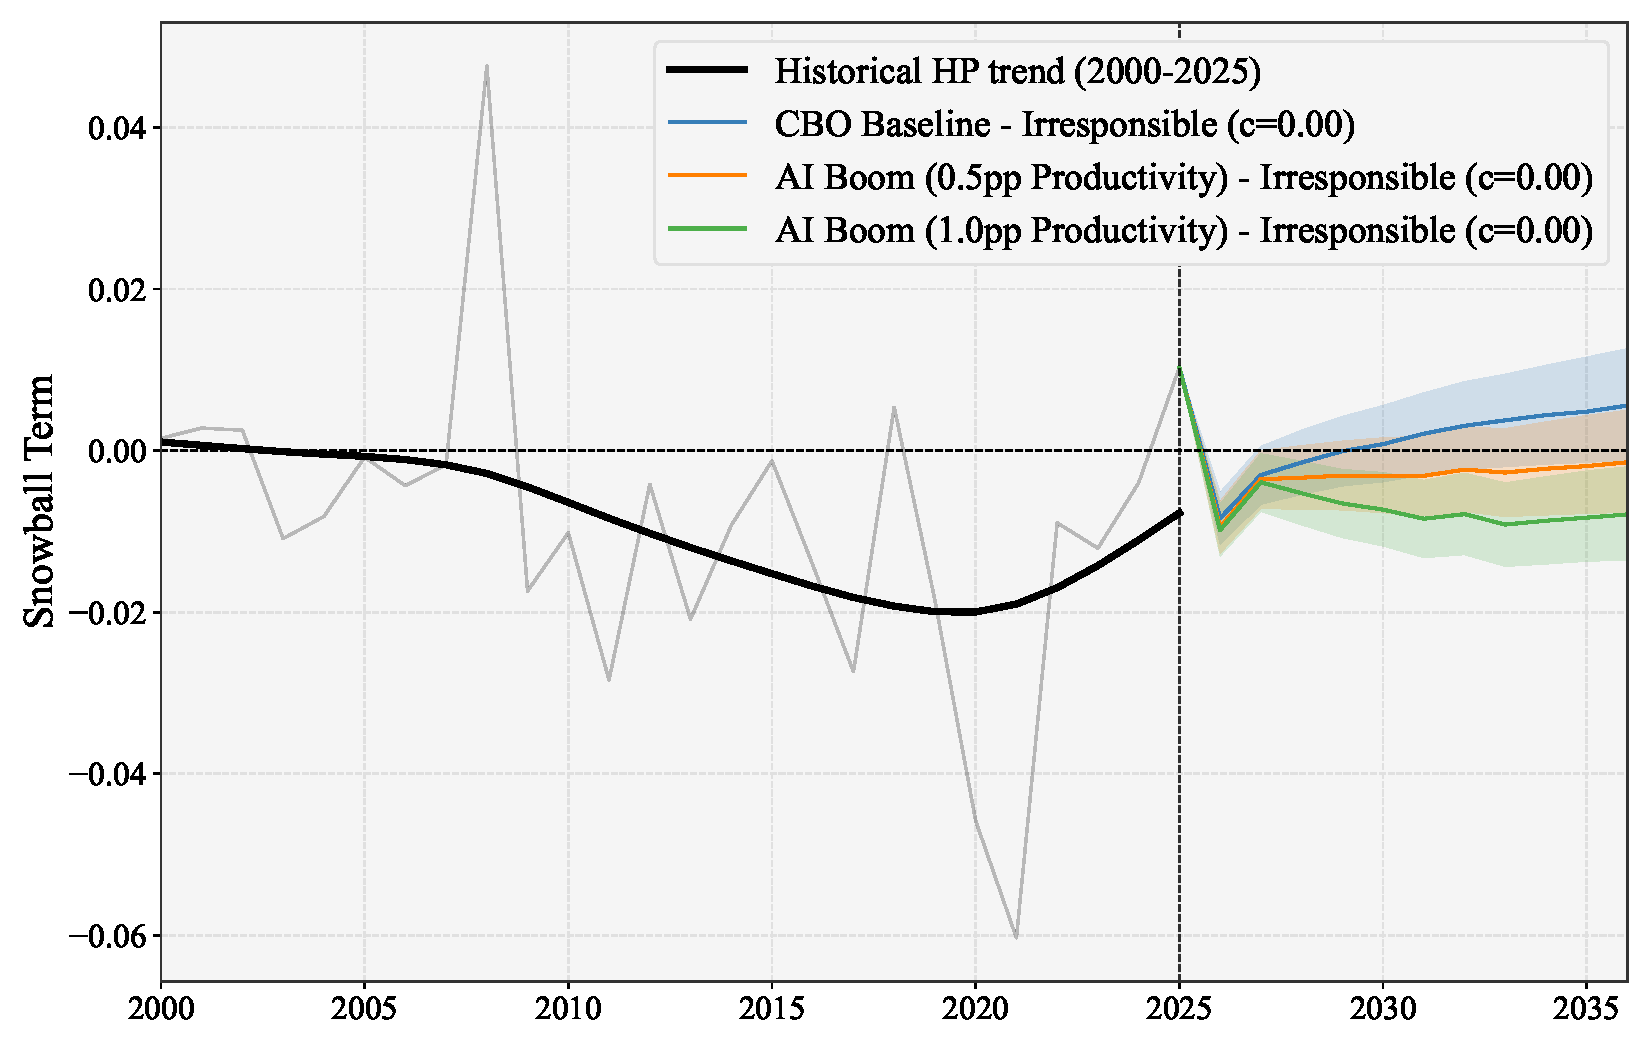
\includegraphics[width=\textwidth]{sdsa_enrichment1_snowball_overlay_ai_booms_0.00.pdf}
	\end{subfigure}
    \caption{Interest-growth contribution to debt accumulation}
    \label{fig:ai_snowball}
\end{figure}
\begin{comment}
\begin{figure}[htbp!]
\centering
	\begin{subfigure}[b]{0.8\textwidth}
		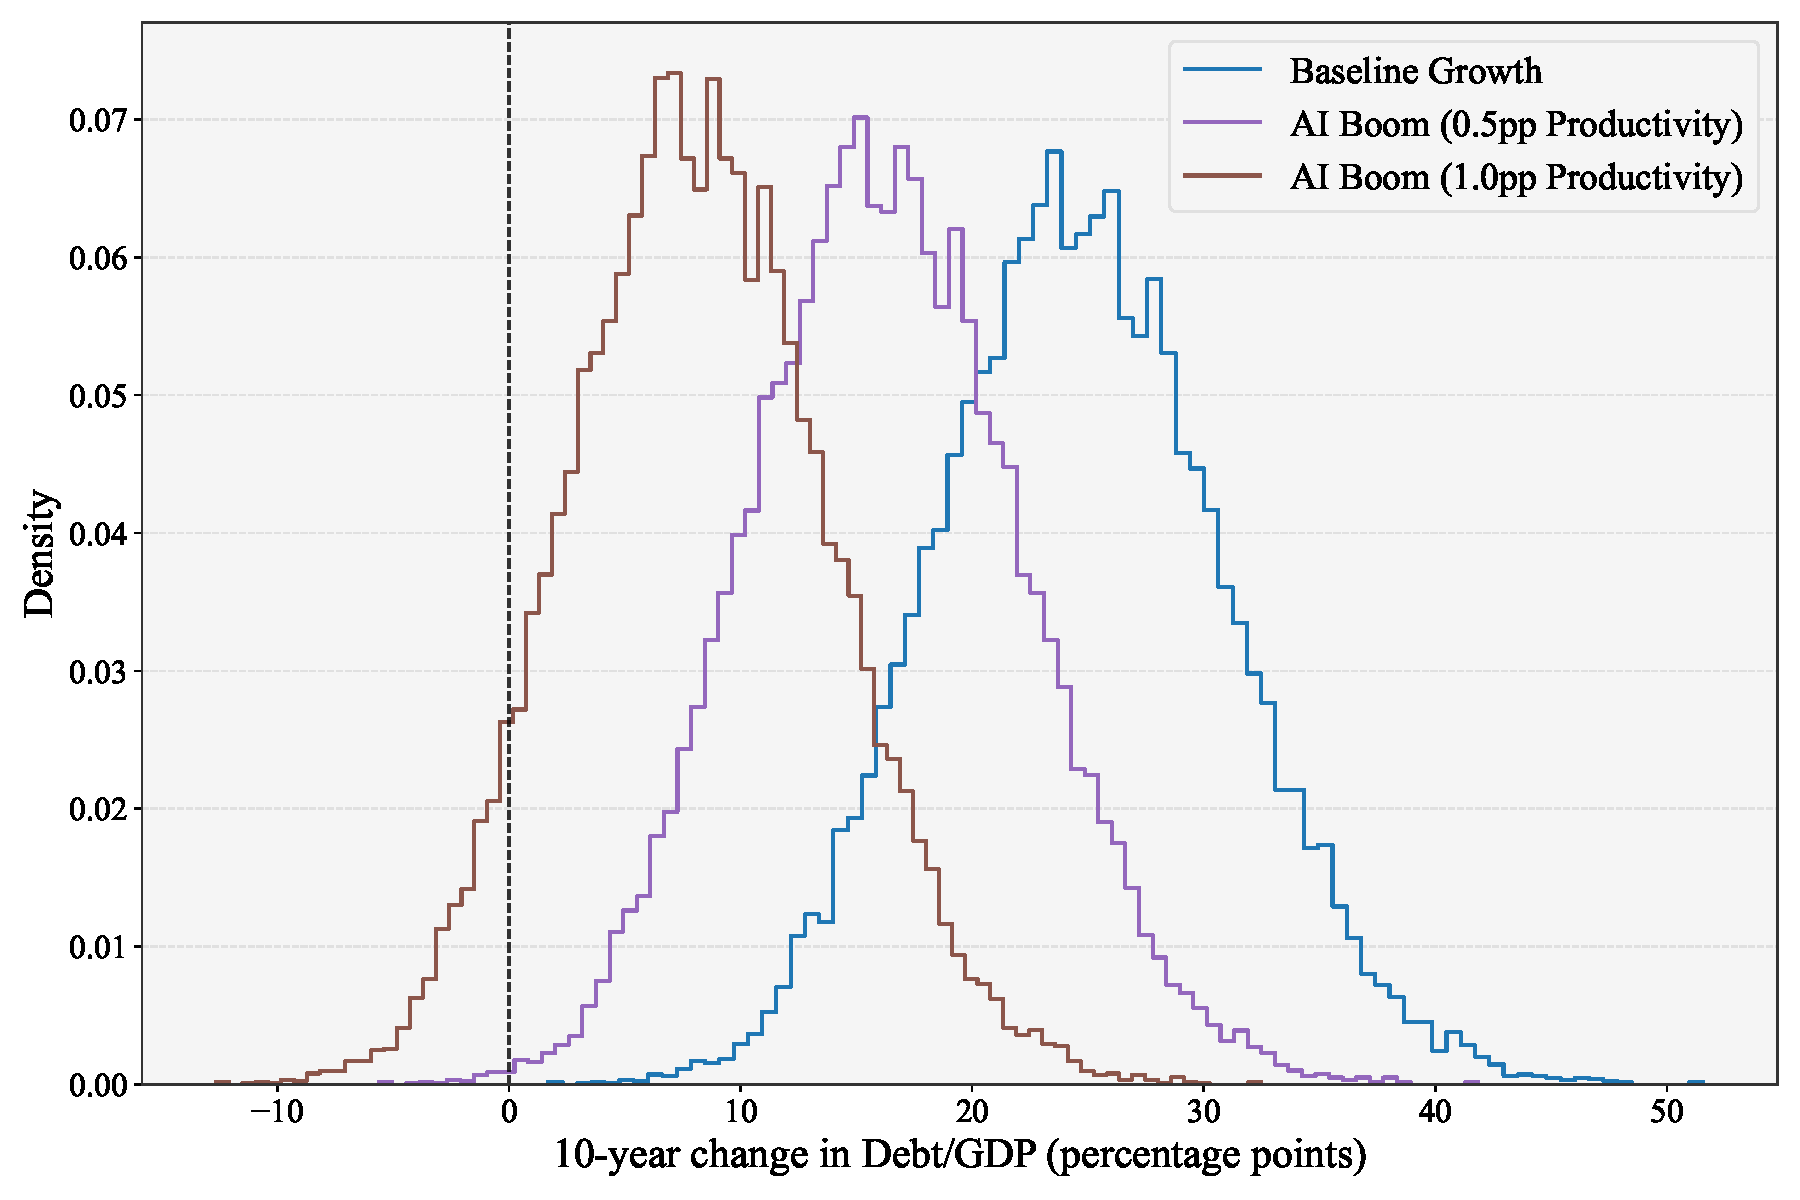
\includegraphics[width=\textwidth]{sdsa_enrichment1_debt_10yr_change_distro_ai_booms_c_0.00.pdf}
	\end{subfigure}
	\caption{Distributions of 10-year changes in debt as a share of GDP (pp)}
    \label{fig:ai_debt_chg_dist}
\end{figure}
\end{comment}

Figure \ref{fig:aa_by_ai_regime} applies our AA framework to these three scenarios. With a 1.0pp boost to productivity, the model implies $AA_t \leq 0$ in the median projection --- i.e., debt stabilization does not require any primary balance tightening. With a 0.5pp boost, the median required primary balance tightening is 1.4 percentage points of GDP. Consolidations of this order are not unprecedented when phased in over several years, having occurred outside of the highly irregular periods of the dot com bubble and post-GFC consolidation. However, our concern in this scenario is concentrated in the upper tail of outcomes, where negative economic shocks could still imply historically large required adjustments.

\begin{figure}[htbp!]
\centering
    \begin{subfigure}[b]{0.95\textwidth}
        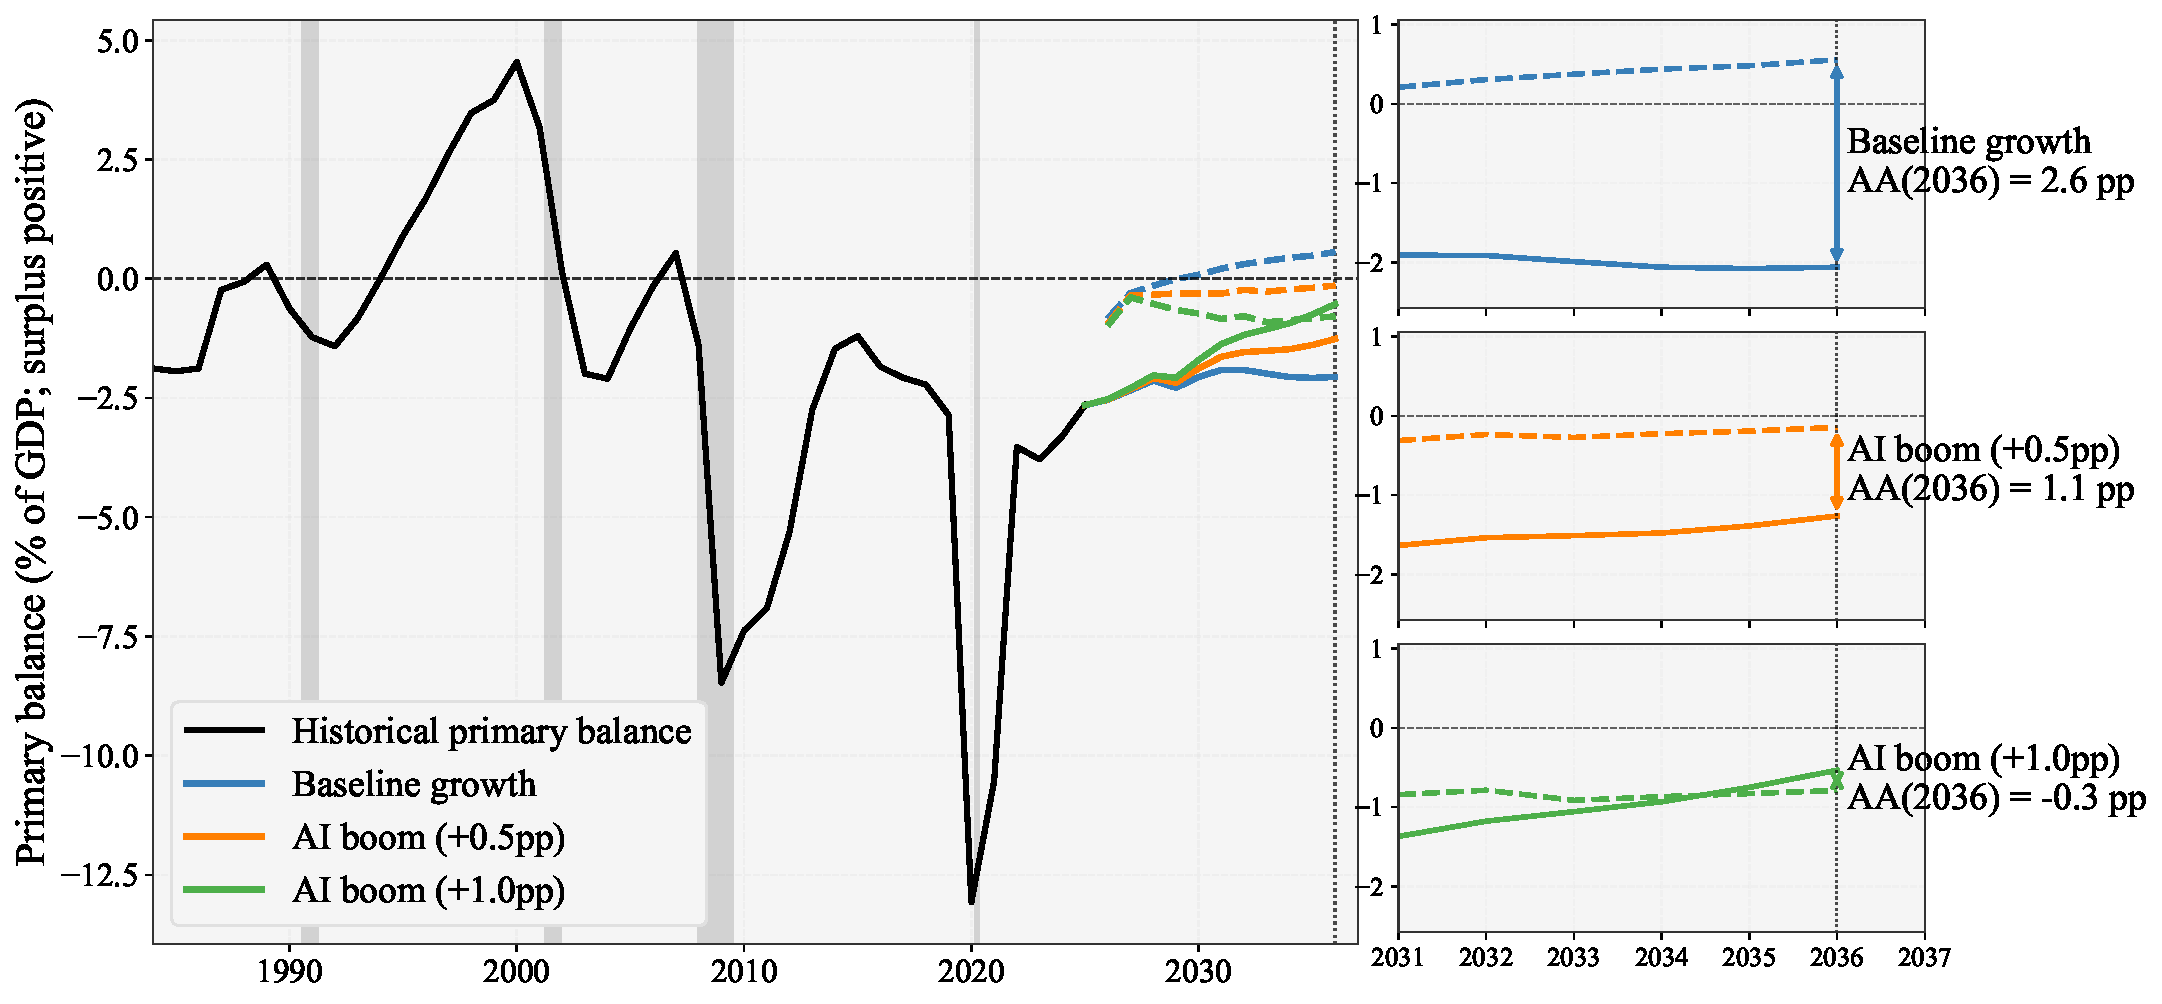
\includegraphics[width=\textwidth]{sdsa_primary_balance_story_popouts_ai_c_0_00.pdf}
    \end{subfigure}
    \caption{Debt-stabilizing primary balance adjustments by AI growth scenario}
    \label{fig:aa_by_ai_regime}
    \begin{minipage}{0.95\textwidth}
    \footnotesize
    \vspace{0.5em}
    \textit{Note:} The dashed lines represent the primary balance required to stabilize the debt (per Equation \ref{eq:stab_balance}). The solid lines illustrate the projected actual primary balance. The difference between the dashed and solid lines in 2035 is annotated and referred to as the required Ahistorical Adjustment (AA).
    \end{minipage}
\end{figure}
\FloatBarrier

\section{Strengths and Weaknesses of our Model}

Any model involves tradeoffs and the simplification of reality. In our model, which we view as a starting point, we have opted to emphasize first principles and model straightforward, easily-interpretable laws of motion for $r$, $g$, $s$, and $b$. This straightforwardness is a strength; we believe that this model is more easily digestible to policymakers than other complex (and also deeply helpful) macroeconomic models and, given that the goal of this exercise is to quantify debt sustainability in a way helpful for policymakers with direct control over our fiscal situation, we consider this a strength --- even if this simplification comes, in part, at the expense of model richness.

Additionally, the model gives us full control over the mean and distribution of the future path of our key macroeconomic variables $r$, $s$, and $g$. This means that we can use as the first moment of any of these variables projections from external sources; if a bill is proposed, and sources such as the CBO or Yale Budget Lab score these proposed policies on their fiscal/growth/interest rate effects, we can very easily construct counterfactual debt paths that allow us to compare across differing policy baselines. Importantly, this also allows us to model what would happen if, as an example, with the election of a new President in 2028, $c$ went from 0 to 0.15 (i.e., Congress continues its fiscal recklessness until a new administration comes to power, and at that point it returns to its 1984-2003 approach to fiscal matters).

One weakness of our model, as a result of its simplification, is our reliance on linear, independent modeling of $r$, $g$, and $s$ (although we do allow for some feedback between $r$ and $s$). We know that the economy is deeply interconnected; changes in $b$ will result in crowding-out which will not only raise $r$ but also, as a result of higher borrowing costs, lower $g$. Our model accounts (in a simplistic way) for this first step in crowding-out; however, we would have to  enrich our current framework to break out interest rate effects separately into 1) effects on the policy / federal funds rate and 2) private borrowing rates, each of which would presumably affect growth differently. Thus, while the (infamous) findings of Reinhart and Rogoff have been debunked, there is no consensus on the relationship between $b$ and $g$ --- meaning it is unclear whether by excluding any causal effect of $b$ on $g$ we risk over- or under-estimating the severity of debt unsustainability \parencite{rahman2019does}.

Furthermore, our model does not take a stance on whether the relationship between debt and interest rates (represented by the coefficient $\beta_r$) will fundamentally change in the future; this remains open speculation as we continue to hurtle into uncharted fiscal waters, but it is certainly possible that in instances of a debt spiral, the relationship between $b$ and $r$ is not linear but instead exponential. 

One final weakness is that our model does not include the granularity to model changes in the composition of outstanding debt. For example, we make no distinction between the government issuing long-term Treasuries or short-term Treasuries to fund itself; instead, we model a fixed and time-invariant parameter $\sigma$ which captures the relative strength of the past average interest rate (intended to reflect the average interest rate across all outstanding debt) in determining the future average interest rate. This lack of enrichment prevents our \textit{accurate} projection of debt servicing as a share of GDP (hence our reliance on the curvature of the debt path, which we believe captures in effect the same phenomenon).

What we would like to emphasize is that none of these weaknesses are fundamental to our model; instead, they require enrichments to the template we've laid down and we encourage alterations to this framework to incorporate more non-linear, interrelated, and complex relationships to further improve this model over time.

\section{Appendix}

\subsection{Previous Estimates of Debt's Effect on Interest Rates}
\begin{table}[htbp!]
\centering
\resizebox{\textwidth}{!}{%
\begin{tabular}{|l|l|l|l|l|}
\hline
\textbf{Source} & \textbf{Estimation Period} & \textbf{\begin{tabular}[c]{@{}l@{}}Effect of 1 pct. pt.\\ increase in debt/GDP\\ (basis points)\end{tabular}} & \textbf{Methodology} & \textbf{\begin{tabular}[c]{@{}l@{}}Term Premium or\\ Expected Short-Rate\end{tabular}} \\ \hline
Engen and Hubbard (2004) & 1976–2003 & 3 bps & OLS and VAR & both \\ \hline
Gale and Orszag (2004) & 1976–2004 & 4–6 bps & OLS & both \\ \hline
Kinoshita (2006) & 1971–2004, international data & 4–5 bps & Panel regression & both \\ \hline
Laubach (2009) & 1976–2006 & 3–4 bps & OLS & both \\ \hline
Chadha et al. (2013) & 1986–2008 & 2 bps & OLS & both \\ \hline
Gamber and Seliski (2019) & 1976–2017 & 2–3 bps & OLS & both \\ \hline
Coenen et al. (2012) & N/A & 1 bp & \begin{tabular}[c]{@{}l@{}}Calibrated\\ structural model\end{tabular} & Expected short-rate ($r^*$) \\ \hline
Mian et al. (2022) & N/A & 1–2 bps & \begin{tabular}[c]{@{}l@{}}Calibrated\\ structural model\end{tabular} & Expected short-rate ($r^*$) \\ \hline
Li and Wei (2013)\textsuperscript{*} & 1994–2007 & 6 bps & \begin{tabular}[c]{@{}l@{}}Estimated term\\ structure model\end{tabular} & Term premium \\ \hline
\end{tabular}%
}
\caption{Estimates of the effect of a 1 percentage point increase in debt-to-GDP on interest rates ($\beta_r$)}
\label{tab:debt_gdp_interest_effect}
\end{table}

\subsection{Detailed Explanation of Modeling $r$}
\label{sec:detailed_explanation_r}

Below we include the regression results from estimating Equation \ref{eq:r_estimation}, under three sample specifications: 1) entire sample, 2) pre-GFC, and 3) post-GFC:
\begin{table}
\begin{center}
\begin{tabular}{llll}
\hline
               & Full sample & Post-GFC & Pre-GFC  \\
\hline
const          & -0.008      & -0.038   & -0.005   \\
               & (0.021)     & (0.037)  & (0.025)  \\
\textbf{d\_b\_lag} ($\mathbf{\beta_r}$)      & \textbf{0.017*}      & \textbf{0.013}    &  \textbf{0.016}    \\
               & (0.009)     & (0.010)  & (0.047)  \\
d\_b\_lag2     & -0.001      & 0.001    & 0.001    \\
               & (0.007)     & (0.006)  & (0.038)  \\
d\_gap         & -0.017      & 0.018    & -0.031   \\
               & (0.021)     & (0.015)  & (0.034)  \\
d\_primary     & 0.015       & 0.019    & 0.018    \\
               & (0.011)     & (0.012)  & (0.039)  \\
\textbf{d\_r\_lag} ($\mathbf{\rho}$)     & \textbf{0.158**}     & \textbf{0.151}    &  \textbf{0.152*}   \\
               & (0.071)     & (0.121)  & (0.085)  \\
               \hline \\
R-squared      & 0.032       & 0.043    & 0.030    \\
N              & 219         & 66       & 148      \\
\hline
\end{tabular}
\caption{ACM 10y term premium: First differences (HAC SEs)}
\label{tab:r_estimation_results}
\end{center}
\end{table}

\subsection{Detailed Explanation of Modeling $s$}
\label{sec:detailed_explanation_s}

To illustrate how $c$ works in our model, we can evaluate the two extreme cases, either where $c = 0$ or where $c = 1$:
\begin{gather}
c = 0 \rightarrow s_t = (1-c)a_{st} + c\left(\frac{r^{av}_t - g_t}{1 + g_t}\right)b_{t-1} + e_t^s = a_{st} + e_t^s \\
c = 1 \rightarrow s_t = (1-c)a_{st} + c\left(\frac{r^{av}_t - g_t}{1 + g_t}\right)b_{t-1} + e_t^s = \left(\frac{r^{av}_t - g_t}{1 + g_t}\right)b_{t-1} + e_t^s
\end{gather}

We ultimately adopt three values for $c$: 0 (total irresponsibility, matching findings by \textcite{auerbach2025robust}), 0.15 (a return to pre-2003 fiscal restraint), and 0.3. 

\subsection{CBO-Modeled Growth Gains from AI Productivity Boom}

Figure \ref{fig:aug_ai_boom_comp} compares the \href{https://www.cbo.gov/publication/61332}{CBO-modeled} AI productivity boom-induced growth rate vs. the baseline projected growth rate.

\begin{figure}[hbpt!]
\centering
    \begin{subfigure}[b]{0.8\textwidth}
        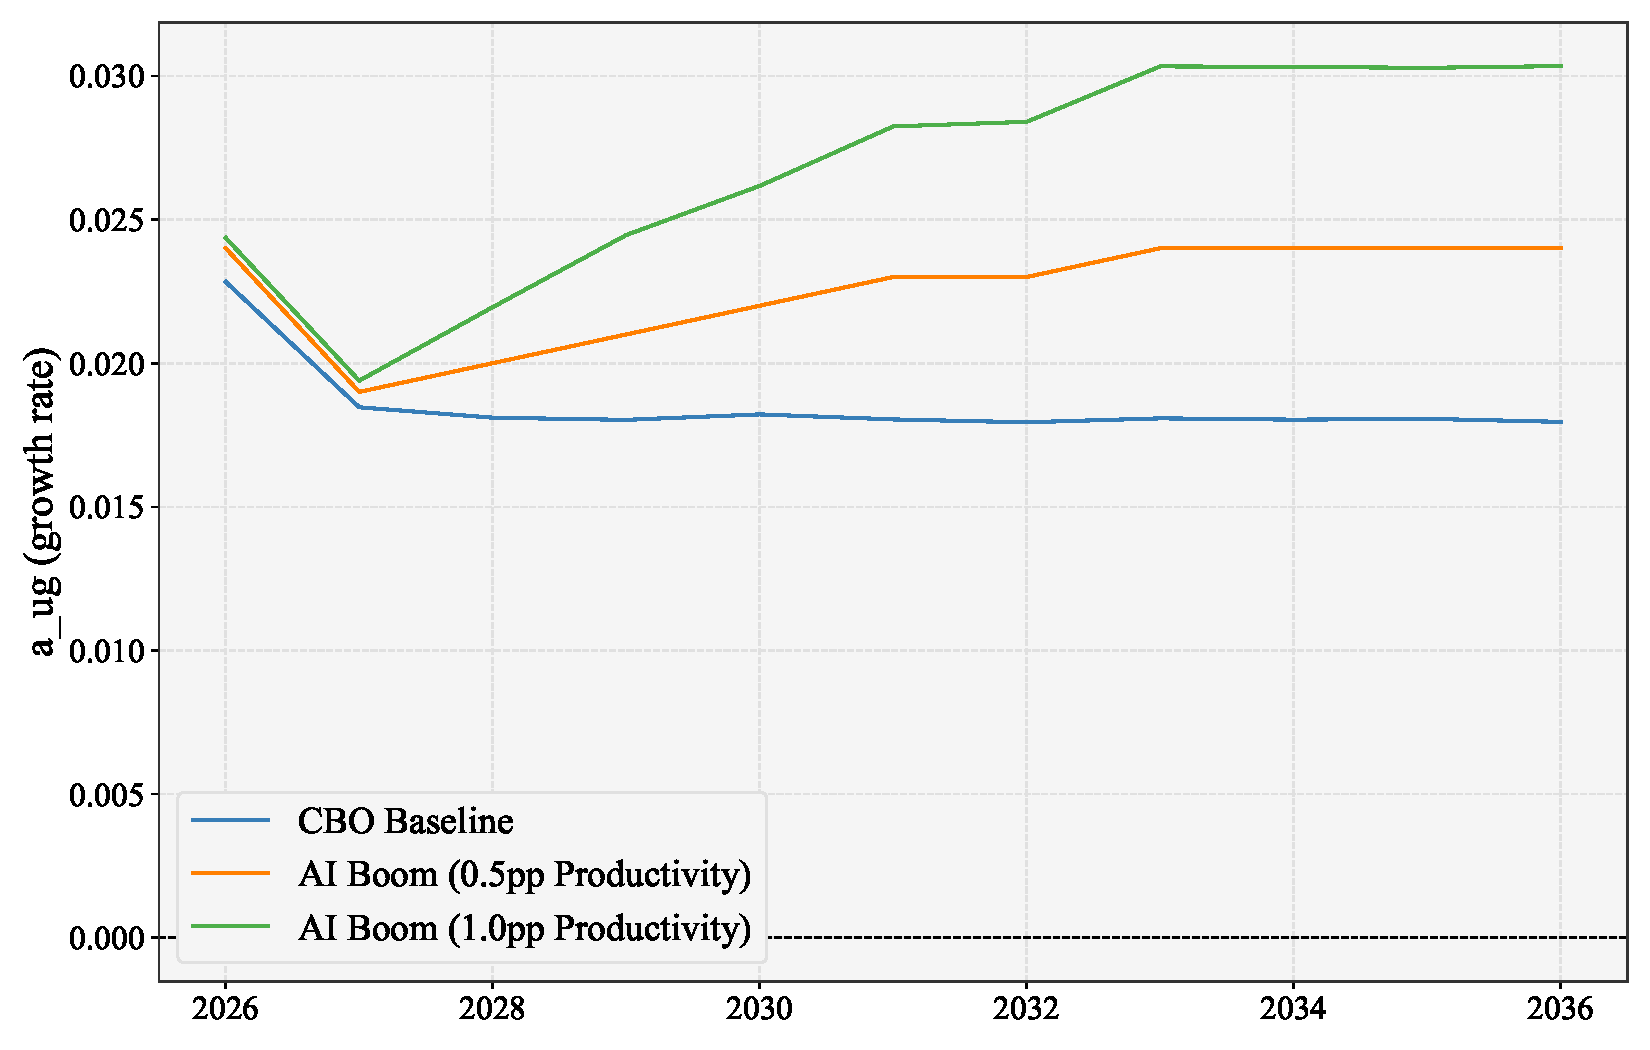
\includegraphics[width=\textwidth]{sdsa_enrichment1_a_ug_paths_ai_booms.pdf}
    \end{subfigure}
    \caption{CBO AI boom and baseline growth rate projections}
    \label{fig:aug_ai_boom_comp}
\end{figure}

\clearpage

\printbibliography

\end{document}